\section{Calculating the Sensor Distance}
The way the experiment is constructed makes it difficult to accurately
measure the distance between the imaging sensor and the focal spot.
However, with knowledge of the angle in which the sensor is tilted, this
distance can be extracted \textit{a posteriori} from measuring the shape
of the light falling on the sensor.
\begin{figure}
\centering
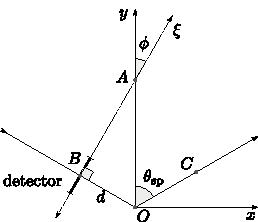
\includegraphics[keepaspectratio,scale=1.25]{figures/hyperbolageoa.pdf}
\caption{Geometry for determining the sensor distance $d$.}
\label{fig:propgeo}
\end{figure}

Consider the experimental geometry.  Light from scattered SPPs eminates as
a cone and is imaged by a planar sensor.  This is by definition a conic
section, with the SPP light cone as the cone and the sensor as the cutting
plane.  Following, the shape of the light on the sensor will be either a
circle, an ellipse, a parabola, or a hyperbola.  In the experimental setup
we can easily set things up such that sensor is fixed
orthogonal to the SPP cone.  The geometrical situation is depicted in
\Figure{fig:propgeo}.  SPPs eminate into the far field from point $O$ at
$\thetasp$.  The detector, which has a finite length, is at $B$ and is
orthogonal to $\overline{OB}$ at an angle $\phi=\pi/2-\thetasp$ with respect to
the normal vector from the prism surface $\overline{OA}$.  Because
$\phi<\thetasp$ and $\thetasp>\pi/2$, lines $\overline{BA}$ and $\overline{OC}$ never
intersect. The resulting shape is a hyperbola.  We wish to determine, given
the parameters of the hyperbolic section, the distance between the focal
spot and the sensor $d$.  

We denote the coordinates of the sensor as $(\xi,y)$.  Here we have the
following relationships
\begin{align}
x &= \xi \cos \thetasp\\
r &= \left(d \sec \thetasp + \xi \sin \thetasp\right) \tan\thetasp
\end{align}
and
\begin{equation}
x^2+y^2=r^2
\end{equation}
Note $d \sec\thetasp$ is the length of $\overline{OA}$.  These two sets of
equations can be combined to obtain
\begin{equation}
\xi^2 \left(\cos ^2\thetasp-\sin ^2\thetasp \tan
^2\thetasp\right)+2 \xi d \tan ^3\thetasp+y^2=d^2 \tan
^2\thetasp \sec ^2\thetasp
\end{equation}
Which, after a bit of algebra, can be solved for $\xi$, taking
the positive root
\begin{equation}
\xi(y) = \frac{4 \sqrt{2} \sqrt{-2 y^2 \cos 2 \thetasp  \cos ^6\thetasp +d^2
\cos ^6\thetasp -d^2 \cos 2 \thetasp  \cos^6\thetasp}-2 d \sin 2 \thetasp
+d \sin 4 \thetasp }{2 \left(2 \cos 2 \thetasp +\cos 4 \thetasp +1\right)}
\label{eqn:conic02}
\end{equation}

To find the offset, we solve the above minimum and find $\xi(y=0) = 4 d
\sec\thetasp$, subtracting this from \Equation{eqn:conic02}.  The remaining
equation is then solved for $d$.
\begin{align}
d =& \Biggl(-4 \sqrt{2} \Bigl(\delta^2 \sin ^2\thetasp \cos
^4\thetasp+\delta^2 \sin ^2\thetasp \cos \thetasp \cos ^4\thetasp-4 y^2 \\
   & \sin ^2\thetasp \cos ^5\thetasp-6 y^2 \sin ^2\thetasp
     \cos ^4\thetasp-16 y^2 \sin ^2\thetasp \cos \thetasp\\
  & \cos ^4\thetasp+4 y^2 \sin ^2\thetasp \cos \thetasp
    \cos ^4\thetasp-8 y^2 \sin ^2\thetasp \cos \thetasp \cos
    ^4\thetasp\Bigr)^{1/2}\\
&-2 \delta\sin \thetasp-4 \delta \sin 3 \thetasp+\delta  \sin \thetasp-4 \delta \sin \thetasp\Biggr)\\
&\cdot\Bigl(4 \left(2 \cos \thetasp+3 \cos \thetasp-3 \cos \thetasp+\cos 5 \thetasp-2 \cos \thetasp-1\right)\Bigr)^{-1}
\end{align}


$\delta$ is the distance the cone goes up at the coordinate $y$.  All you
need is the pixel dimensions and this equation will get you what you want.
